\documentclass[11pt]{article}
\usepackage[textwidth=18.0cm, textheight=23.0cm, top=2.0cm]{geometry}
\usepackage{pst-all}
\usepackage{amssymb}
\usepackage{tikz}
\usepackage{underscore}\begin{document}
\pagestyle{empty}


ClassName: \underline{\textbf{Class_08.2bp-2}}
\par
BinSize: \underline{\textbf{100 × 100}}
\par
ReduceSize: \underline{\textbf{100 × 100}}
\par
TypeNum: \underline{\textbf{20}}
\par
Num: \underline{\textbf{20}}
\par
OutS: \underline{\textbf{50000}}
\par
InS: \underline{\textbf{44102}}
\par
Rate: \underline{\textbf{0.882}}
\par
UB: \underline{\textbf{5}}
\par
LB0: \underline{\textbf{5}}
\par
LB: \underline{\textbf{5}}
\par
LBWithCut: \underline{\textbf{5}}
\par
NodeCut: \underline{\textbf{0}}
\par
ExtendedNodeCnt: \underline{\textbf{1}}
\par
GenNodeCnt: \underline{\textbf{1}}
\par
PrimalNode: \underline{\textbf{0}}
\par
ColumnCount: \underline{\textbf{5}}
\par
TotalCutCount: \underline{\textbf{0}}
\par
RootCutCount: \underline{\textbf{0}}
\par
LPSolverCnt: \underline{\textbf{1}}
\par
PricingSolverCnt: \underline{\textbf{0}}
\par
BranchAndBoundNum: \underline{\textbf{1}}
\par
isOpt: \underline{\textbf{true}}
\par
TimeOnInitSolution: \underline{\textbf{0.000 s}}
\par
TimeOnPrimal: \underline{\textbf{0.000 s}}
\par
TimeOnPricing: \underline{\textbf{0.000 s}}
\par
TimeOnRmp: \underline{\textbf{0.062 s}}
\par
TotalTime: \underline{\textbf{0.125 s}}
\par
\newpage


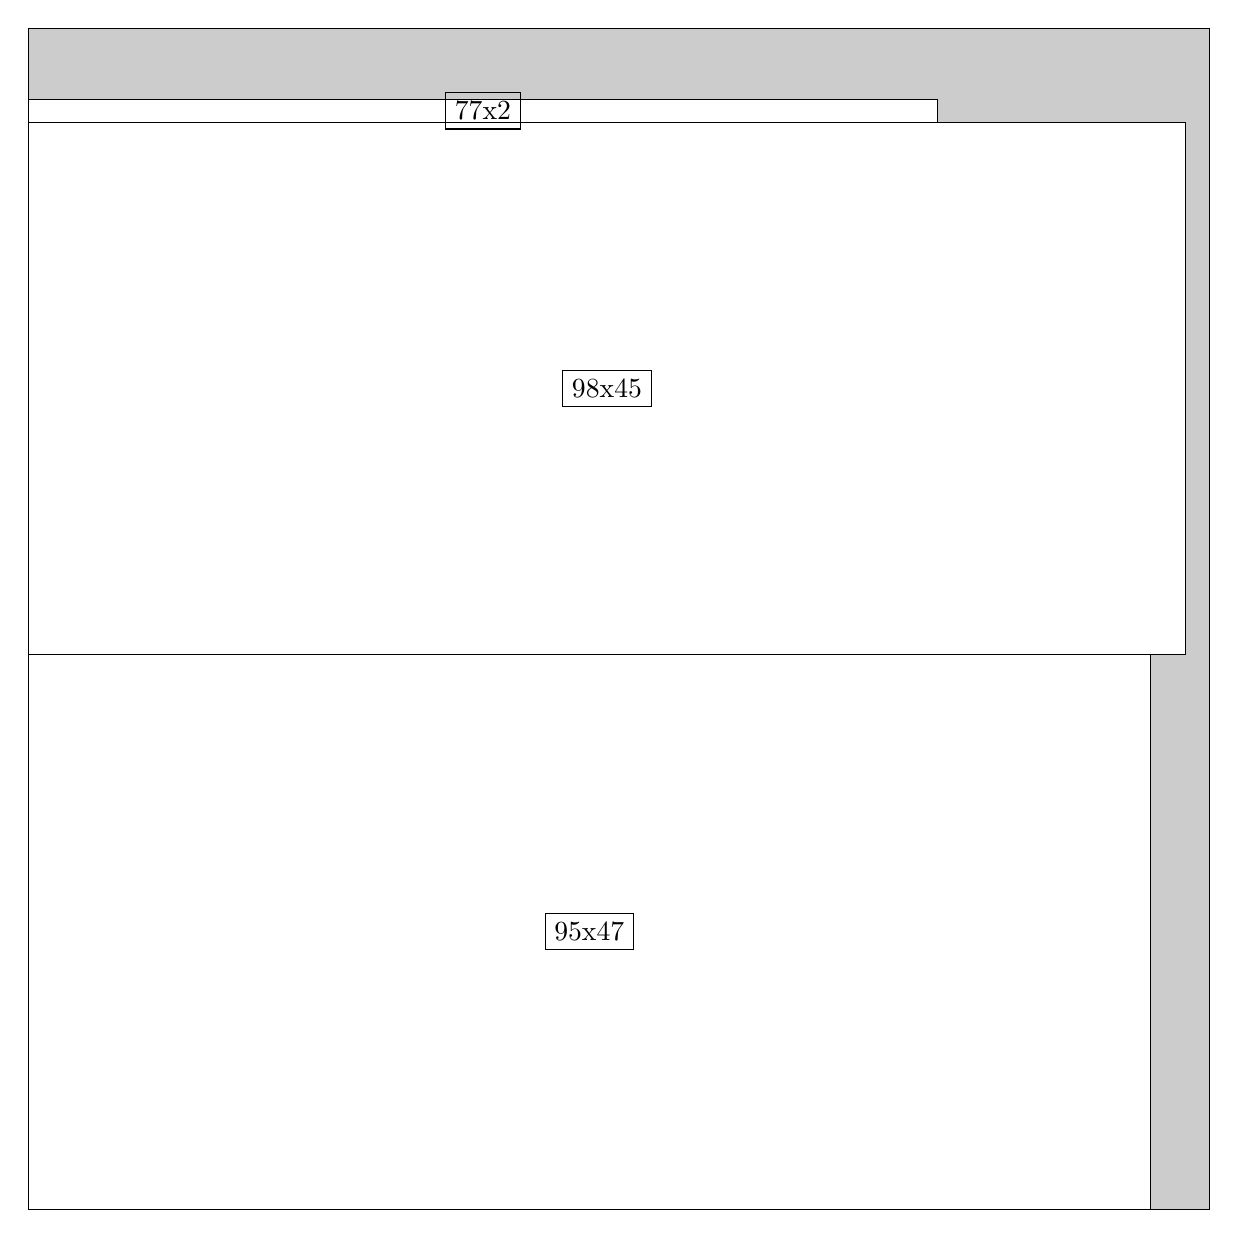
\begin{tikzpicture}[shorten >=1pt,scale=1.0,every node/.style={scale=1.0},->]
\tikzstyle{vertex}=[circle,fill=black!25,minimum size=14pt,inner sep=0pt]
\filldraw[fill=gray!40!white, draw=black] (0,0) rectangle (15.0,15.0);
\foreach \name/\x/\y/\w/\h in {95x47/0.0/0.0/14.25/7.05,98x45/0.0/7.05/14.7/6.75,77x2/0.0/13.799999999999999/11.549999999999999/0.3}
\filldraw[fill=white!40!white, draw=black] (\x,\y) rectangle node[draw] (\name) {\name} ++(\w,\h);
\end{tikzpicture}


w =95 , h =47 , x =0 , y =0 , v =4465
\par
w =98 , h =45 , x =0 , y =47 , v =4410
\par
w =77 , h =2 , x =0 , y =92 , v =154
\par
\newpage


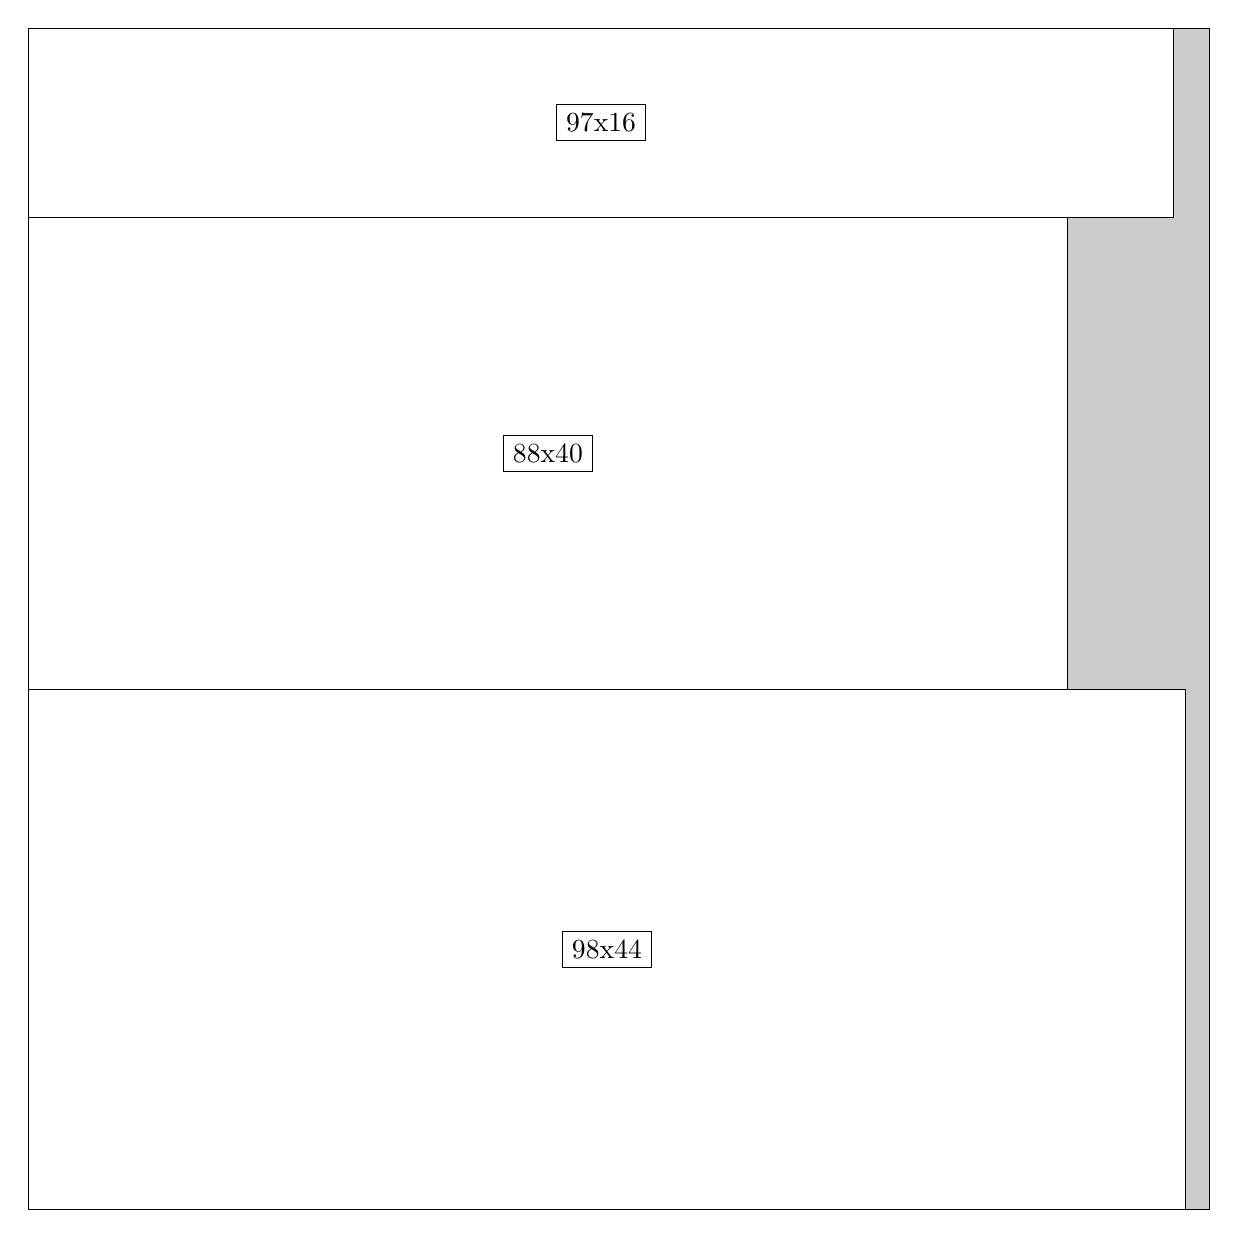
\begin{tikzpicture}[shorten >=1pt,scale=1.0,every node/.style={scale=1.0},->]
\tikzstyle{vertex}=[circle,fill=black!25,minimum size=14pt,inner sep=0pt]
\filldraw[fill=gray!40!white, draw=black] (0,0) rectangle (15.0,15.0);
\foreach \name/\x/\y/\w/\h in {98x44/0.0/0.0/14.7/6.6,88x40/0.0/6.6/13.2/6.0,97x16/0.0/12.6/14.549999999999999/2.4}
\filldraw[fill=white!40!white, draw=black] (\x,\y) rectangle node[draw] (\name) {\name} ++(\w,\h);
\end{tikzpicture}


w =98 , h =44 , x =0 , y =0 , v =4312
\par
w =88 , h =40 , x =0 , y =44 , v =3520
\par
w =97 , h =16 , x =0 , y =84 , v =1552
\par
\newpage


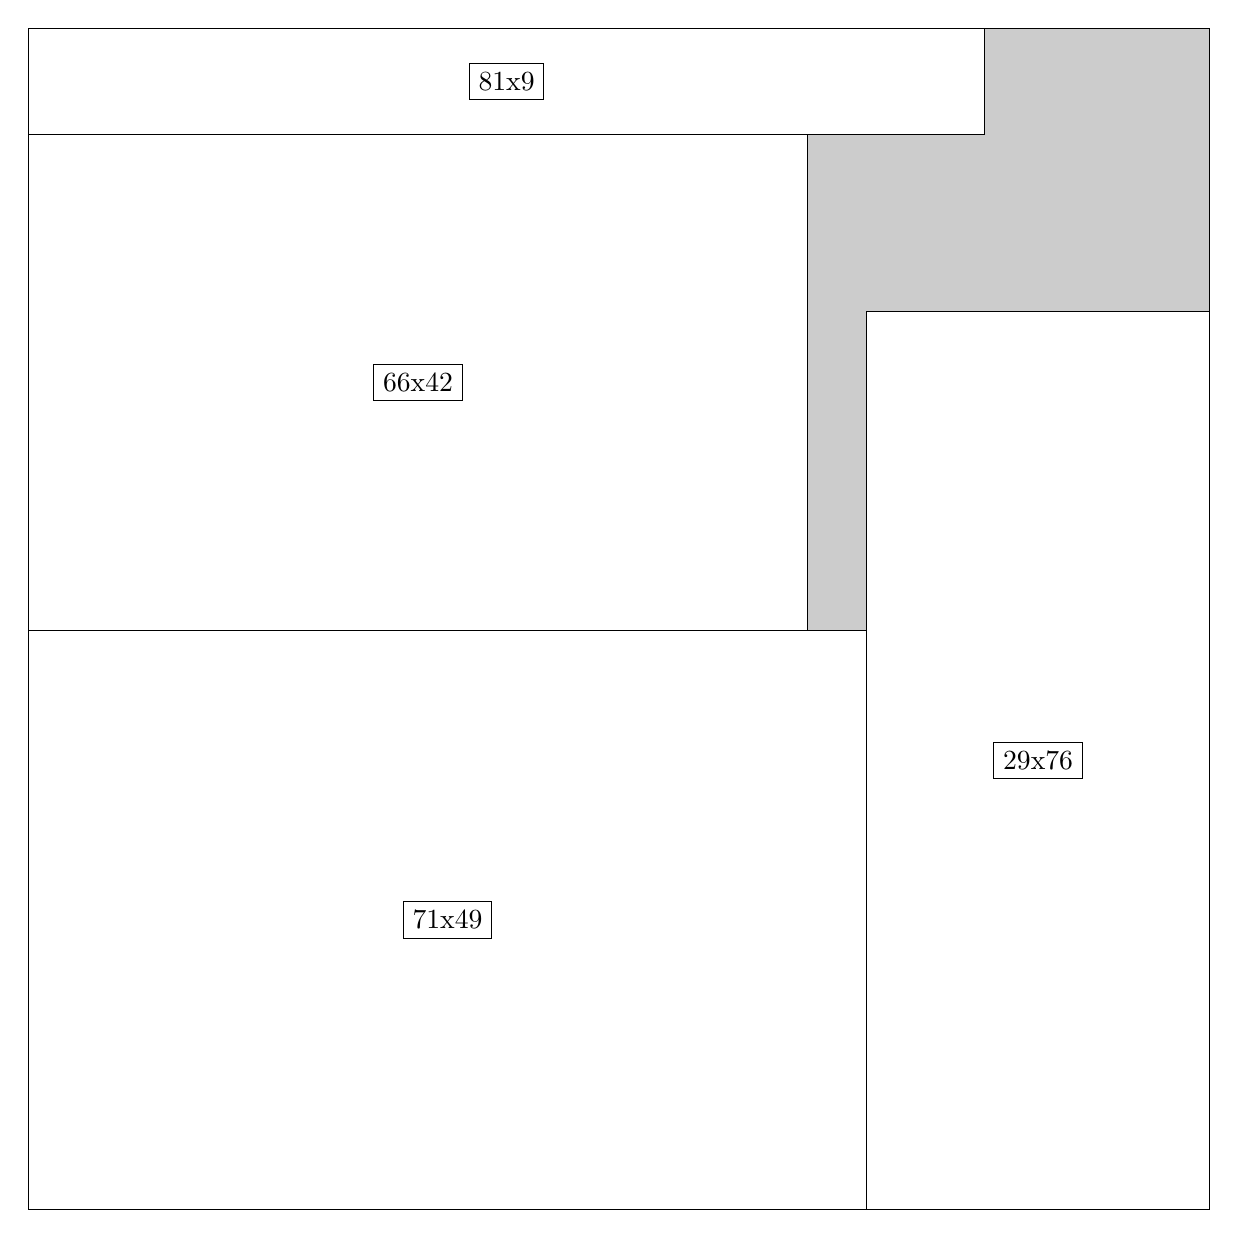
\begin{tikzpicture}[shorten >=1pt,scale=1.0,every node/.style={scale=1.0},->]
\tikzstyle{vertex}=[circle,fill=black!25,minimum size=14pt,inner sep=0pt]
\filldraw[fill=gray!40!white, draw=black] (0,0) rectangle (15.0,15.0);
\foreach \name/\x/\y/\w/\h in {71x49/0.0/0.0/10.65/7.35,66x42/0.0/7.35/9.9/6.3,29x76/10.65/0.0/4.35/11.4,81x9/0.0/13.65/12.15/1.3499999999999999}
\filldraw[fill=white!40!white, draw=black] (\x,\y) rectangle node[draw] (\name) {\name} ++(\w,\h);
\end{tikzpicture}


w =71 , h =49 , x =0 , y =0 , v =3479
\par
w =66 , h =42 , x =0 , y =49 , v =2772
\par
w =29 , h =76 , x =71 , y =0 , v =2204
\par
w =81 , h =9 , x =0 , y =91 , v =729
\par
\newpage


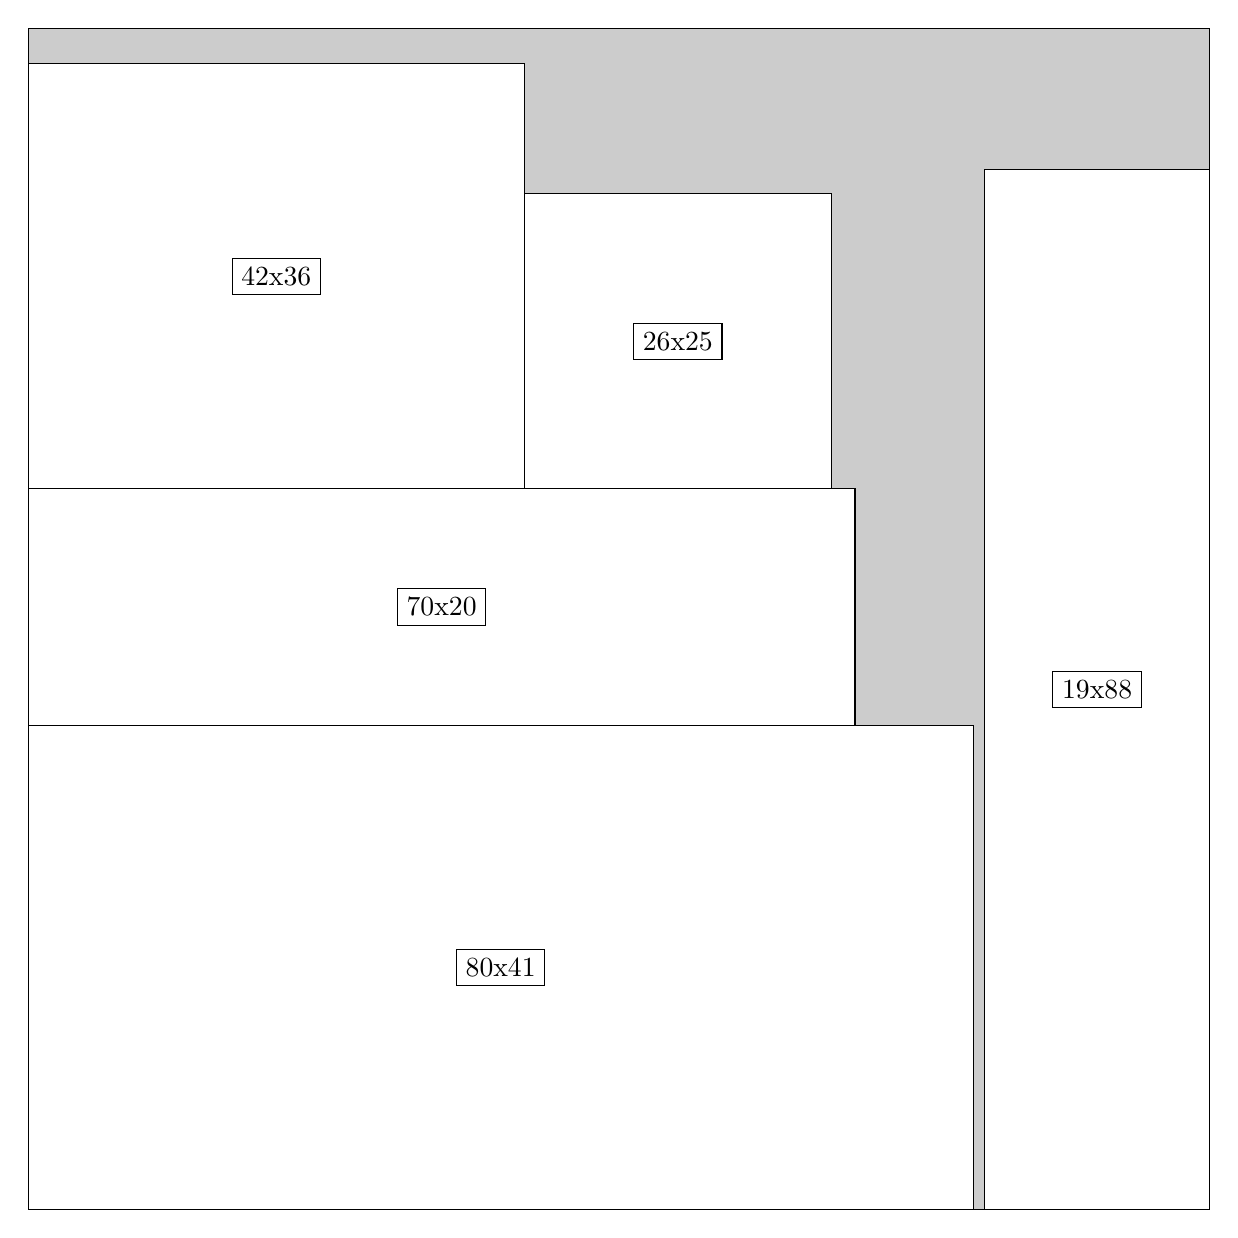
\begin{tikzpicture}[shorten >=1pt,scale=1.0,every node/.style={scale=1.0},->]
\tikzstyle{vertex}=[circle,fill=black!25,minimum size=14pt,inner sep=0pt]
\filldraw[fill=gray!40!white, draw=black] (0,0) rectangle (15.0,15.0);
\foreach \name/\x/\y/\w/\h in {80x41/0.0/0.0/12.0/6.1499999999999995,70x20/0.0/6.1499999999999995/10.5/3.0,19x88/12.15/0.0/2.85/13.2,42x36/0.0/9.15/6.3/5.3999999999999995,26x25/6.3/9.15/3.9/3.75}
\filldraw[fill=white!40!white, draw=black] (\x,\y) rectangle node[draw] (\name) {\name} ++(\w,\h);
\end{tikzpicture}


w =80 , h =41 , x =0 , y =0 , v =3280
\par
w =70 , h =20 , x =0 , y =41 , v =1400
\par
w =19 , h =88 , x =81 , y =0 , v =1672
\par
w =42 , h =36 , x =0 , y =61 , v =1512
\par
w =26 , h =25 , x =42 , y =61 , v =650
\par
\newpage


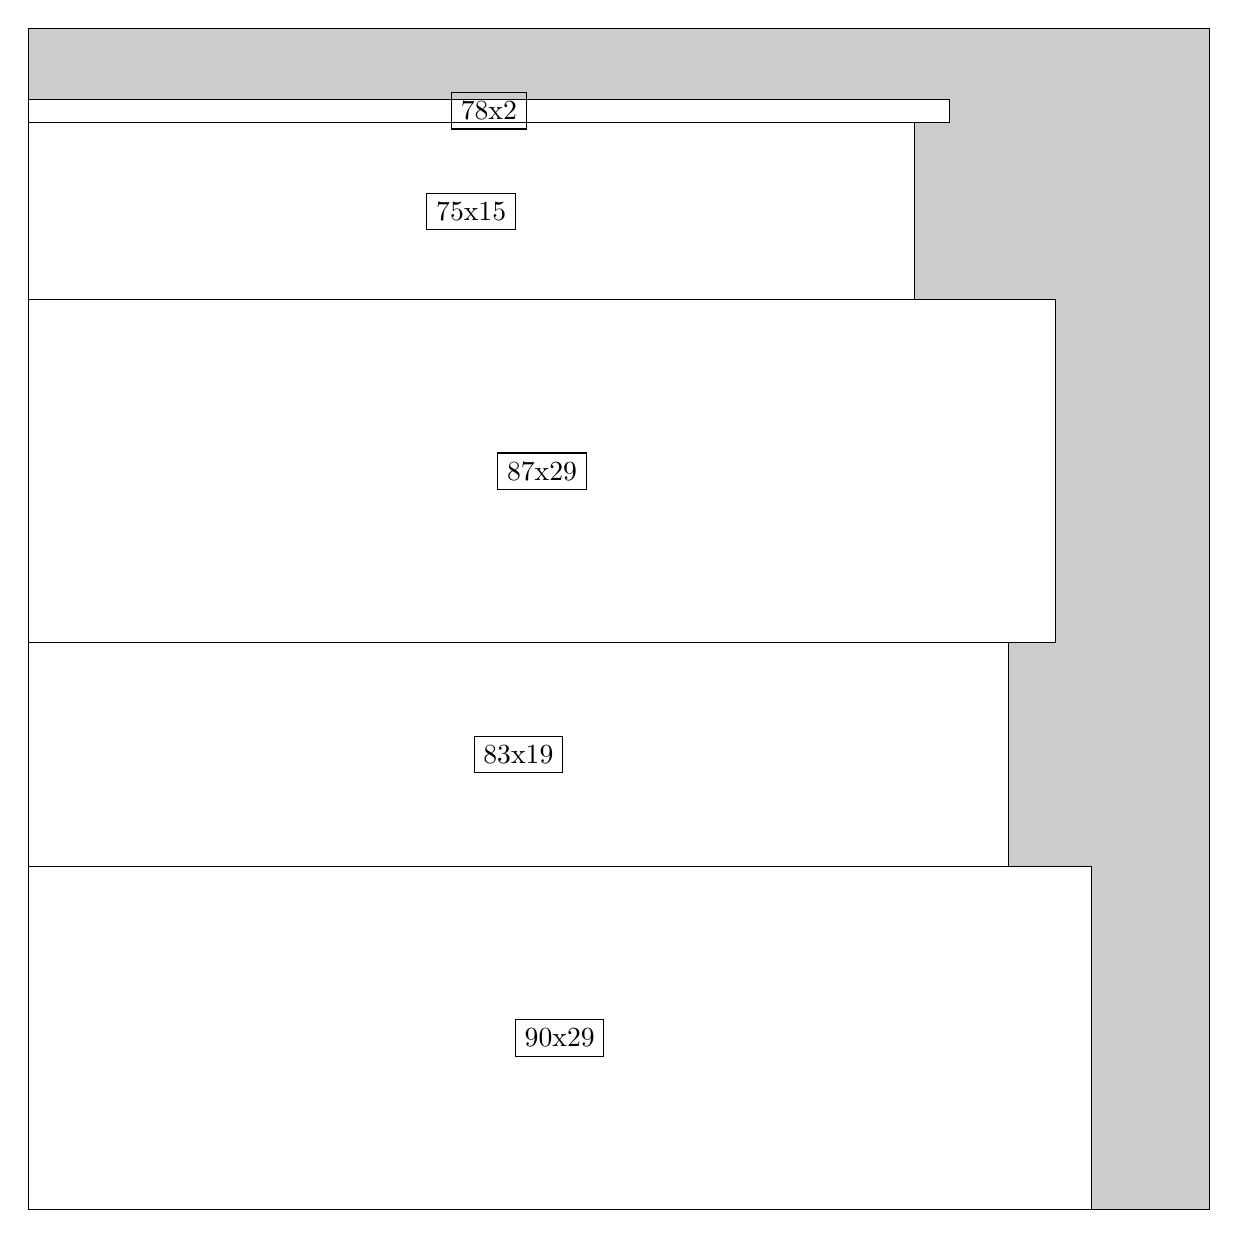
\begin{tikzpicture}[shorten >=1pt,scale=1.0,every node/.style={scale=1.0},->]
\tikzstyle{vertex}=[circle,fill=black!25,minimum size=14pt,inner sep=0pt]
\filldraw[fill=gray!40!white, draw=black] (0,0) rectangle (15.0,15.0);
\foreach \name/\x/\y/\w/\h in {90x29/0.0/0.0/13.5/4.35,83x19/0.0/4.35/12.45/2.85,87x29/0.0/7.199999999999999/13.049999999999999/4.35,75x15/0.0/11.549999999999999/11.25/2.25,78x2/0.0/13.799999999999999/11.7/0.3}
\filldraw[fill=white!40!white, draw=black] (\x,\y) rectangle node[draw] (\name) {\name} ++(\w,\h);
\end{tikzpicture}


w =90 , h =29 , x =0 , y =0 , v =2610
\par
w =83 , h =19 , x =0 , y =29 , v =1577
\par
w =87 , h =29 , x =0 , y =48 , v =2523
\par
w =75 , h =15 , x =0 , y =77 , v =1125
\par
w =78 , h =2 , x =0 , y =92 , v =156
\par
\newpage


\end{document}